\ifx\master\undefined% AUTOCOMPILE
% Allows for individual chapters to be compiled.

% Usage:
% \ifx\master\undefined% AUTOCOMPILE
% Allows for individual chapters to be compiled.

% Usage:
% \ifx\master\undefined% AUTOCOMPILE
% Allows for individual chapters to be compiled.

% Usage:
% \ifx\master\undefined\input{../settings/autocompile}\fi
% (place at start and end of chapter file)

\ifx\noprelim\undefined
    % first time included
    % input preamble files
    \input{../settings/phdsetup}

    \begin{document}
    \def\noprelim{}
\else
    % already included once
    % input post files

    \singlespacing
    \bibliographystyle{../bibliography/expanded}
    \bibliography{../bibliography/references}

    \end{document}
\fi\fi
% (place at start and end of chapter file)

\ifx\noprelim\undefined
    % first time included
    % input preamble files
    % [ USER VARIABLES ]

\def\PHDTITLE {Extensions of the Theory of Computational Mechanics}
\def\PHDAUTHOR{Evan Klose Friis}
\def\PHDSCHOOL{University of California, Davis}

\def\PHDMONTH {June}
\def\PHDYEAR  {2011}
\def\PHDDEPT {Physics}

\def\BSSCHOOL {University of California at San Diego}
\def\BSYEAR   {2005}

\def\PHDCOMMITTEEA{Professor John Conway}
\def\PHDCOMMITTEEB{Professor Robin Erbacher}
\def\PHDCOMMITTEEC{Professor Mani Tripathi}

% [ GLOBAL SETUP ]

\documentclass[letterpaper,oneside,11pt]{report}

\usepackage{calc}
\usepackage{breakcites}
\usepackage[newcommands]{ragged2e}

\usepackage[pdftex]{graphicx}
\usepackage{epstopdf}

%\usepackage{tikz}
%\usetikzlibrary{positioning} % [right=of ...]
%\usetikzlibrary{fit} % [fit= ...]

%\pgfdeclarelayer{background layer}
%\pgfdeclarelayer{foreground layer}
%\pgfsetlayers{background layer,main,foreground layer}

%\newenvironment{wrap}{\noindent\begin{minipage}[t]{\linewidth}\vspace{-0.5\normalbaselineskip}\centering}{\vspace{0.5\normalbaselineskip}\end{minipage}}

%% [Venn diagram environment]
%\newenvironment{venn2}
%{\begin{tikzpicture} [every pin/.style={text=black, text opacity=1.0, pin distance=0.5cm, pin edge={black!60, semithick}},
%% define a new style 'venn'
%venn/.style={circle, draw=black!60, semithick, minimum size = 4cm}]
%
%% create circle and give it external (pin) label
%\node[venn] (X) at (-1,0) [pin={150:$H[X]$}] {};
%\node[venn] (Y) at (1,0) [pin={30:$H[Y]$}] {};
%
%% place labels of the atoms by hand
%\node at (-1.9,0) {$H[X|Y]$};
%\node at (1.9,0) {$H[Y|X]$};
%\node at (0,0) {$I[X;Y]$};}
%{\end{tikzpicture}}

%\newcommand{\wrapmath}[1]{\begin{wrap}\begin{tikzpicture}[every node/.style={inner ysep=0ex, inner xsep=0em}]\node[] {$\displaystyle\begin{aligned} #1\end{aligned}$};\end{tikzpicture}\end{wrap}}

\renewenvironment{abstract}{\chapter*{Abstract}}{}
\renewcommand{\bibname}{Bibliography}
\renewcommand{\contentsname}{Table of Contents}

\makeatletter
\renewcommand{\@biblabel}[1]{\textsc{#1}}
\makeatother

% [ FONT SETTINGS ]

\usepackage[tbtags, intlimits, namelimits]{amsmath}
\usepackage[adobe-utopia]{mathdesign}

\DeclareSymbolFont{pazomath}{OMS}{zplm}{m}{n}
\DeclareSymbolFontAlphabet{\mathcal}{pazomath}
\SetMathAlphabet\mathcal{bold}{OMS}{zplm}{b}{n}

\SetSymbolFont{largesymbols}{normal}{OMX}{zplm}{m}{n}
\SetSymbolFont{largesymbols}{bold}{OMX}{zplm}{m}{n}
\SetSymbolFont{symbols}{normal}{OMS}{zplm}{m}{n}
\SetSymbolFont{symbols}{bold}{OMS}{zplm}{b}{n}

\renewcommand{\sfdefault}{phv}
\renewcommand{\ttdefault}{fvm}

\widowpenalty 8000
\clubpenalty  8000

% [ PAGE LAYOUT ]
\usepackage{geometry}
\geometry{lmargin = 1.5in}
\geometry{rmargin = 1.0in}
\geometry{tmargin = 1.0in}
\geometry{bmargin = 1.0in}

% [ PDF SETTINGS ]

\usepackage[final]{hyperref}
\hypersetup{breaklinks  = true}
\hypersetup{colorlinks  = true}
\hypersetup{linktocpage = false}
\hypersetup{linkcolor   = blue}
\hypersetup{citecolor   = green}
\hypersetup{urlcolor    = black}
\hypersetup{plainpages  = false}
\hypersetup{pageanchor  = true}
\hypersetup{pdfauthor   = {\PHDAUTHOR}}
\hypersetup{pdftitle    = {\PHDTITLE}}
\hypersetup{pdfsubject  = {Dissertation, \PHDSCHOOL}}
\urlstyle{same}

% [ LETTER SPACING ]

\usepackage[final]{microtype}
\microtypesetup{protrusion=compatibility}
\microtypesetup{expansion=false}

\newcommand{\upper}[1]{\MakeUppercase{#1}}
\let\lsscshape\scshape

\ifcase\pdfoutput\else\microtypesetup{letterspace=15}
\renewcommand{\scshape}{\lsscshape\lsstyle}
\renewcommand{\upper}[1]{\textls[50]{\MakeUppercase{#1}}}\fi

% [ LINE SPACING ]

\usepackage[doublespacing]{setspace}
\renewcommand{\displayskipstretch}{0.0}

\setlength{\parskip   }{0em}
\setlength{\parindent }{2em}

% [ TABLE FORMATTING ]

\usepackage{booktabs}
\setlength{\heavyrulewidth}{1.5\arrayrulewidth}
\setlength{\lightrulewidth}{1.0\arrayrulewidth}
\setlength{\doublerulesep }{2.0\arrayrulewidth}

% [ SECTION FORMATTING ]

\usepackage[largestsep,nobottomtitles*]{titlesec}
\renewcommand{\bottomtitlespace}{0.75in}

\titleformat{\chapter}[display]{\bfseries\huge\singlespacing}{\filleft\textsc{\LARGE \chaptertitlename\ \thechapter}}{-0.2ex}{\titlerule[3pt]\vspace{0.2ex}}[]

\titleformat{\section}{\LARGE}{\S\thesection\hspace{0.5em}}{0ex}{}
\titleformat{\subsection}{\Large}{\S\thesubsection\hspace{0.5em}}{0ex}{}
\titleformat{\subsubsection}{\large}{\thesubsubsection\hspace{0.5em}}{0ex}{}

\titlespacing*{\chapter}{0em}{6ex}{4ex plus 2ex minus 0ex}
\titlespacing*{\section}{0em}{2ex plus 3ex minus 1ex}{0.5ex plus 0.5ex minus 0.5ex}
\titlespacing*{\subsection}{0ex}{2ex plus 3ex minus 1ex}{0ex}
\titlespacing*{\subsubsection}{0ex}{2ex plus 0ex minus 1ex}{0ex}

% [ HEADER SETTINGS ]

\usepackage{fancyhdr}

\setlength{\headheight}{\normalbaselineskip}
\setlength{\footskip  }{0.5in}
\setlength{\headsep   }{0.5in-\headheight}

\fancyheadoffset[R]{0.5in}
\renewcommand{\headrulewidth}{0pt}
\renewcommand{\footrulewidth}{0pt}

\newcommand{\pagebox}{\parbox[r][\headheight][t]{0.5in}{\hspace\fill\thepage}}

\newcommand{\prelimheaders}{\ifx\prelim\undefined\renewcommand{\thepage}{\textit{\roman{page}}}\fancypagestyle{plain}{\fancyhf{}\fancyfoot[L]{\makebox[\textwidth-0.5in]{\thepage}}}\pagestyle{plain}\def\prelim{}\fi}

\newcommand{\normalheaders}{\renewcommand{\thepage}{\arabic{page}}\fancypagestyle{plain}{\fancyhf{}\fancyhead[R]{\pagebox}}\pagestyle{plain}}

\normalheaders{}

% [ CUSTOM COMMANDS ]

\newcommand{\signaturebox}[1]{\multicolumn{1}{p{4in}}{\vspace{3ex}}\\\midrule #1\\}

%\input{../includes/cmechabbrev}

% [some math stuff - maybe stick in sep file]
\usepackage{amsthm}
\usepackage{amscd}
\theoremstyle{plain}    \newtheorem{Lem}{Lemma}
\theoremstyle{plain}    \newtheorem*{ProLem}{Proof}
\theoremstyle{plain} 	\newtheorem{Cor}{Corollary}
\theoremstyle{plain} 	\newtheorem*{ProCor}{Proof}
\theoremstyle{plain} 	\newtheorem{The}{Theorem}
\theoremstyle{plain} 	\newtheorem*{ProThe}{Proof}
\theoremstyle{plain} 	\newtheorem{Prop}{Proposition}
\theoremstyle{plain} 	\newtheorem*{ProProp}{Proof}
\theoremstyle{plain} 	\newtheorem*{Conj}{Conjecture}
\theoremstyle{plain}	\newtheorem*{Rem}{Remark}
\theoremstyle{plain}	\newtheorem*{Def}{Definition} 
\theoremstyle{plain}	\newtheorem*{Not}{Notation}

% [uniform figure scaling - maybe this is not a good idea]
\def\figscale{.7}
\def\lscale{1.0}

% [FIX ME! - red makes it easier to spot]
\newcommand{\FIX}[1]{\textbf{\textcolor{red}{#1}}}


    \begin{document}
    \def\noprelim{}
\else
    % already included once
    % input post files

    \singlespacing
    \bibliographystyle{../bibliography/expanded}
    \bibliography{../bibliography/references}

    \end{document}
\fi\fi
% (place at start and end of chapter file)

\ifx\noprelim\undefined
    % first time included
    % input preamble files
    % [ USER VARIABLES ]

\def\PHDTITLE {Extensions of the Theory of Computational Mechanics}
\def\PHDAUTHOR{Evan Klose Friis}
\def\PHDSCHOOL{University of California, Davis}

\def\PHDMONTH {June}
\def\PHDYEAR  {2011}
\def\PHDDEPT {Physics}

\def\BSSCHOOL {University of California at San Diego}
\def\BSYEAR   {2005}

\def\PHDCOMMITTEEA{Professor John Conway}
\def\PHDCOMMITTEEB{Professor Robin Erbacher}
\def\PHDCOMMITTEEC{Professor Mani Tripathi}

% [ GLOBAL SETUP ]

\documentclass[letterpaper,oneside,11pt]{report}

\usepackage{calc}
\usepackage{breakcites}
\usepackage[newcommands]{ragged2e}

\usepackage[pdftex]{graphicx}
\usepackage{epstopdf}

%\usepackage{tikz}
%\usetikzlibrary{positioning} % [right=of ...]
%\usetikzlibrary{fit} % [fit= ...]

%\pgfdeclarelayer{background layer}
%\pgfdeclarelayer{foreground layer}
%\pgfsetlayers{background layer,main,foreground layer}

%\newenvironment{wrap}{\noindent\begin{minipage}[t]{\linewidth}\vspace{-0.5\normalbaselineskip}\centering}{\vspace{0.5\normalbaselineskip}\end{minipage}}

%% [Venn diagram environment]
%\newenvironment{venn2}
%{\begin{tikzpicture} [every pin/.style={text=black, text opacity=1.0, pin distance=0.5cm, pin edge={black!60, semithick}},
%% define a new style 'venn'
%venn/.style={circle, draw=black!60, semithick, minimum size = 4cm}]
%
%% create circle and give it external (pin) label
%\node[venn] (X) at (-1,0) [pin={150:$H[X]$}] {};
%\node[venn] (Y) at (1,0) [pin={30:$H[Y]$}] {};
%
%% place labels of the atoms by hand
%\node at (-1.9,0) {$H[X|Y]$};
%\node at (1.9,0) {$H[Y|X]$};
%\node at (0,0) {$I[X;Y]$};}
%{\end{tikzpicture}}

%\newcommand{\wrapmath}[1]{\begin{wrap}\begin{tikzpicture}[every node/.style={inner ysep=0ex, inner xsep=0em}]\node[] {$\displaystyle\begin{aligned} #1\end{aligned}$};\end{tikzpicture}\end{wrap}}

\renewenvironment{abstract}{\chapter*{Abstract}}{}
\renewcommand{\bibname}{Bibliography}
\renewcommand{\contentsname}{Table of Contents}

\makeatletter
\renewcommand{\@biblabel}[1]{\textsc{#1}}
\makeatother

% [ FONT SETTINGS ]

\usepackage[tbtags, intlimits, namelimits]{amsmath}
\usepackage[adobe-utopia]{mathdesign}

\DeclareSymbolFont{pazomath}{OMS}{zplm}{m}{n}
\DeclareSymbolFontAlphabet{\mathcal}{pazomath}
\SetMathAlphabet\mathcal{bold}{OMS}{zplm}{b}{n}

\SetSymbolFont{largesymbols}{normal}{OMX}{zplm}{m}{n}
\SetSymbolFont{largesymbols}{bold}{OMX}{zplm}{m}{n}
\SetSymbolFont{symbols}{normal}{OMS}{zplm}{m}{n}
\SetSymbolFont{symbols}{bold}{OMS}{zplm}{b}{n}

\renewcommand{\sfdefault}{phv}
\renewcommand{\ttdefault}{fvm}

\widowpenalty 8000
\clubpenalty  8000

% [ PAGE LAYOUT ]
\usepackage{geometry}
\geometry{lmargin = 1.5in}
\geometry{rmargin = 1.0in}
\geometry{tmargin = 1.0in}
\geometry{bmargin = 1.0in}

% [ PDF SETTINGS ]

\usepackage[final]{hyperref}
\hypersetup{breaklinks  = true}
\hypersetup{colorlinks  = true}
\hypersetup{linktocpage = false}
\hypersetup{linkcolor   = blue}
\hypersetup{citecolor   = green}
\hypersetup{urlcolor    = black}
\hypersetup{plainpages  = false}
\hypersetup{pageanchor  = true}
\hypersetup{pdfauthor   = {\PHDAUTHOR}}
\hypersetup{pdftitle    = {\PHDTITLE}}
\hypersetup{pdfsubject  = {Dissertation, \PHDSCHOOL}}
\urlstyle{same}

% [ LETTER SPACING ]

\usepackage[final]{microtype}
\microtypesetup{protrusion=compatibility}
\microtypesetup{expansion=false}

\newcommand{\upper}[1]{\MakeUppercase{#1}}
\let\lsscshape\scshape

\ifcase\pdfoutput\else\microtypesetup{letterspace=15}
\renewcommand{\scshape}{\lsscshape\lsstyle}
\renewcommand{\upper}[1]{\textls[50]{\MakeUppercase{#1}}}\fi

% [ LINE SPACING ]

\usepackage[doublespacing]{setspace}
\renewcommand{\displayskipstretch}{0.0}

\setlength{\parskip   }{0em}
\setlength{\parindent }{2em}

% [ TABLE FORMATTING ]

\usepackage{booktabs}
\setlength{\heavyrulewidth}{1.5\arrayrulewidth}
\setlength{\lightrulewidth}{1.0\arrayrulewidth}
\setlength{\doublerulesep }{2.0\arrayrulewidth}

% [ SECTION FORMATTING ]

\usepackage[largestsep,nobottomtitles*]{titlesec}
\renewcommand{\bottomtitlespace}{0.75in}

\titleformat{\chapter}[display]{\bfseries\huge\singlespacing}{\filleft\textsc{\LARGE \chaptertitlename\ \thechapter}}{-0.2ex}{\titlerule[3pt]\vspace{0.2ex}}[]

\titleformat{\section}{\LARGE}{\S\thesection\hspace{0.5em}}{0ex}{}
\titleformat{\subsection}{\Large}{\S\thesubsection\hspace{0.5em}}{0ex}{}
\titleformat{\subsubsection}{\large}{\thesubsubsection\hspace{0.5em}}{0ex}{}

\titlespacing*{\chapter}{0em}{6ex}{4ex plus 2ex minus 0ex}
\titlespacing*{\section}{0em}{2ex plus 3ex minus 1ex}{0.5ex plus 0.5ex minus 0.5ex}
\titlespacing*{\subsection}{0ex}{2ex plus 3ex minus 1ex}{0ex}
\titlespacing*{\subsubsection}{0ex}{2ex plus 0ex minus 1ex}{0ex}

% [ HEADER SETTINGS ]

\usepackage{fancyhdr}

\setlength{\headheight}{\normalbaselineskip}
\setlength{\footskip  }{0.5in}
\setlength{\headsep   }{0.5in-\headheight}

\fancyheadoffset[R]{0.5in}
\renewcommand{\headrulewidth}{0pt}
\renewcommand{\footrulewidth}{0pt}

\newcommand{\pagebox}{\parbox[r][\headheight][t]{0.5in}{\hspace\fill\thepage}}

\newcommand{\prelimheaders}{\ifx\prelim\undefined\renewcommand{\thepage}{\textit{\roman{page}}}\fancypagestyle{plain}{\fancyhf{}\fancyfoot[L]{\makebox[\textwidth-0.5in]{\thepage}}}\pagestyle{plain}\def\prelim{}\fi}

\newcommand{\normalheaders}{\renewcommand{\thepage}{\arabic{page}}\fancypagestyle{plain}{\fancyhf{}\fancyhead[R]{\pagebox}}\pagestyle{plain}}

\normalheaders{}

% [ CUSTOM COMMANDS ]

\newcommand{\signaturebox}[1]{\multicolumn{1}{p{4in}}{\vspace{3ex}}\\\midrule #1\\}

%%%% macros fro standard references
%\eqref provided by amsmath
\newcommand{\figref}[1]{Fig.~\ref{#1}}
\newcommand{\tableref}[1]{Table~\ref{#1}}
\newcommand{\refcite}[1]{Ref.~\cite{#1}}

% Abbreviations from CMPPSS:

\newcommand{\eM}     {\mbox{$\epsilon$-machine}}
\newcommand{\eMs}    {\mbox{$\epsilon$-machines}}
\newcommand{\EM}     {\mbox{$\epsilon$-Machine}}
\newcommand{\EMs}    {\mbox{$\epsilon$-Machines}}
\newcommand{\eT}     {\mbox{$\epsilon$-transducer}}
\newcommand{\eTs}    {\mbox{$\epsilon$-transducers}}
\newcommand{\ET}     {\mbox{$\epsilon$-Transducer}}
\newcommand{\ETs}    {\mbox{$\epsilon$-Transducers}}

% Processes and sequences

\newcommand{\Process}{\mathcal{P}}

\newcommand{\ProbMach}{\Prob_{\mathrm{M}}}
\newcommand{\Lmax}   { {L_{\mathrm{max}}}}
\newcommand{\MeasAlphabet}	{\mathcal{A}}
% Original
%\newcommand{\MeasSymbol}   { {S} }
%\newcommand{\meassymbol}   { {s} }
% New symbol
\newcommand{\MeasSymbol}   { {X} }
\newcommand{\meassymbol}   { {x} }
\newcommand{\BiInfinity}	{ \overleftrightarrow {\MeasSymbol} }
\newcommand{\biinfinity}	{ \overleftrightarrow {\meassymbol} }
\newcommand{\Past}	{ \overleftarrow {\MeasSymbol} }
\newcommand{\past}	{ {\overleftarrow {\meassymbol}} }
\newcommand{\pastprime}	{ {\past}^{\prime}}
\newcommand{\Future}	{ \overrightarrow{\MeasSymbol} }
\newcommand{\future}	{ \overrightarrow{\meassymbol} }
\newcommand{\futureprime}	{ {\future}^{\prime}}
\newcommand{\PastPrime}	{ {\Past}^{\prime}}
\newcommand{\FuturePrime}	{ {\overrightarrow{\meassymbol}}^\prime }
\newcommand{\PastDblPrime}	{ {\overleftarrow{\meassymbol}}^{\prime\prime} }
\newcommand{\FutureDblPrime}	{ {\overrightarrow{\meassymbol}}^{\prime\prime} }
\newcommand{\pastL}	{ {\overleftarrow {\meassymbol}}{}^L }
\newcommand{\PastL}	{ {\overleftarrow {\MeasSymbol}}{}^L }
\newcommand{\PastLt}	{ {\overleftarrow {\MeasSymbol}}_t^L }
\newcommand{\PastLLessOne}	{ {\overleftarrow {\MeasSymbol}}^{L-1} }
\newcommand{\futureL}	{ {\overrightarrow{\meassymbol}}{}^L }
\newcommand{\FutureL}	{ {\overrightarrow{\MeasSymbol}}{}^L }
\newcommand{\FutureLt}	{ {\overrightarrow{\MeasSymbol}}_t^L }
\newcommand{\FutureLLessOne}	{ {\overrightarrow{\MeasSymbol}}^{L-1} }
\newcommand{\pastLprime}	{ {\overleftarrow {\meassymbol}}^{L^\prime} }
\newcommand{\futureLprime}	{ {\overrightarrow{\meassymbol}}^{L^\prime} }
\newcommand{\AllPasts}	{ { \overleftarrow {\rm {\bf \MeasSymbol}} } }
\newcommand{\AllFutures}	{ \overrightarrow {\rm {\bf \MeasSymbol}} }
\newcommand{\FutureSet}	{ \overrightarrow{\bf \MeasSymbol}}

% Causal states and epsilon-machines
\newcommand{\CausalState}	{ \mathcal{S} }
\newcommand{\CausalStatePrime}	{ {\CausalState}^{\prime}}
\newcommand{\causalstate}	{ \sigma }
\newcommand{\CausalStateSet}	{ \boldsymbol{\CausalState} }
\newcommand{\AlternateState}	{ \mathcal{R} }
\newcommand{\AlternateStatePrime}	{ {\cal R}^{\prime} }
\newcommand{\alternatestate}	{ \rho }
\newcommand{\alternatestateprime}	{ {\rho^{\prime}} }
\newcommand{\AlternateStateSet}	{ \boldsymbol{\AlternateState} }
\newcommand{\PrescientState}	{ \widehat{\AlternateState} }
\newcommand{\prescientstate}	{ \widehat{\alternatestate} }
\newcommand{\PrescientStateSet}	{ \boldsymbol{\PrescientState}}
\newcommand{\CausalEquivalence}	{ {\sim}_{\epsilon} }
\newcommand{\CausalEquivalenceNot}	{ {\not \sim}_{\epsilon}}

\newcommand{\NonCausalEquivalence}	{ {\sim}_{\eta} }
\newcommand{\NextObservable}	{ {\overrightarrow {\MeasSymbol}}^1 }
\newcommand{\LastObservable}	{ {\overleftarrow {\MeasSymbol}}^1 }
%\newcommand{\Prob}		{ {\rm P}}
\newcommand{\Prob}      {\Pr} % use standard command
\newcommand{\ProbAnd}	{ {,\;} }
\newcommand{\LLimit}	{ {L \rightarrow \infty}}
\newcommand{\Cmu}		{C_\mu}
\newcommand{\hmu}		{h_\mu}
\newcommand{\EE}		{{\bf E}}
\newcommand{\Measurable}{{\bf \mu}}

% Process Crypticity
\newcommand{\PC}		{\chi}
\newcommand{\FuturePC}		{\PC^+}
\newcommand{\PastPC}		{\PC^-}
% Causal Irreversibility
\newcommand{\CI}		{\Xi}
\newcommand{\ReverseMap}	{r}
\newcommand{\ForwardMap}	{f}

% Abbreviations from IB:
% None that aren't already in CMPPSS

% Abbreviations from Extensive Estimation:
\newcommand{\EstCausalState}	{\widehat{\CausalState}}
\newcommand{\estcausalstate}	{\widehat{\causalstate}}
\newcommand{\EstCausalStateSet}	{\boldsymbol{\EstCausalState}}
\newcommand{\EstCausalFunc}	{\widehat{\epsilon}}
\newcommand{\EstCmu}		{\widehat{\Cmu}}
\newcommand{\PastLOne}	{{\Past}^{L+1}}
\newcommand{\pastLOne}	{{\past}^{L+1}}

% Abbreviations from $\epsilon$-Transducers:
\newcommand{\InAlphabet}	{ \mathcal{A}}
\newcommand{\insymbol}		{ a}
\newcommand{\OutAlphabet}	{ \mathcal{B}}
\newcommand{\outsymbol}		{ b}
\newcommand{\InputSimple}	{ X}
\newcommand{\inputsimple}	{ x}
\newcommand{\BottleneckVar}	{\tilde{\InputSimple}}
\newcommand{\bottleneckvar}	{\tilde{\inputsimple}}
\newcommand{\InputSpace}	{ \mathbf{\InputSimple}}
\newcommand{\InputBi}	{ \overleftrightarrow {\InputSimple} }
\newcommand{\inputbi}	{ \overleftrightarrow {\inputsimple} }
\newcommand{\InputPast}	{ \overleftarrow {\InputSimple} }
\newcommand{\inputpast}	{ \overleftarrow {\inputsimple} }
\newcommand{\InputFuture}	{ \overrightarrow {\InputSimple} }
\newcommand{\inputfuture}	{ \overrightarrow {\inputsimple} }
\newcommand{\NextInput}	{ {{\InputFuture}^{1}}}
\newcommand{\NextOutput}	{ {\OutputFuture}^{1}}
\newcommand{\OutputSimple}	{ Y}
\newcommand{\outputsimple}	{ y}
\newcommand{\OutputSpace}	{ \mathbf{\OutputSimple}}
\newcommand{\OutputBi}	{ \overleftrightarrow{\OutputSimple} }
\newcommand{\outputbi}	{ \overleftrightarrow{\outputsimple} }
\newcommand{\OutputPast}	{ \overleftarrow{\OutputSimple} }
\newcommand{\outputpast}	{ \overleftarrow{\outputsimple} }
\newcommand{\OutputFuture}	{ \overrightarrow{\OutputSimple} }
\newcommand{\outputfuture}	{ \overrightarrow{\outputsimple} }
\newcommand{\OutputL}	{ {\OutputFuture}^L}
\newcommand{\outputL}	{ {\outputfuture}^L}
\newcommand{\InputLLessOne}	{ {\InputFuture}^{L-1}}
\newcommand{\inputLlessone}	{ {\inputufutre}^{L-1}}
\newcommand{\OutputPastLLessOne}	{{\OutputPast}^{L-1}_{-1}}
\newcommand{\outputpastLlessone}	{{\outputpast}^{L-1}}
\newcommand{\OutputPastLessOne}	{{\OutputPast}_{-1}}
\newcommand{\outputpastlessone}	{{\outputpast}_{-1}}
\newcommand{\OutputPastL}	{{\OutputPast}^{L}}
\newcommand{\OutputLPlusOne}	{ {\OutputFuture}^{L+1}}
\newcommand{\outputLplusone}	{ {\outputfutre}^{L+1}}
\newcommand{\InputPastL}	{{\InputPast}^{L}}
\newcommand{\inputpastL}	{{\inputpast}^{L}}
\newcommand{\JointPast}	{{(\InputPast,\OutputPast)}}
\newcommand{\jointpast}	{{(\inputpast,\outputpast)}}
\newcommand{\jointpastone}	{{(\inputpast_1,\outputpast_1)}}
\newcommand{\jointpasttwo}	{{(\inputpast_2,\outputpast_2)}}
\newcommand{\jointpastprime} {{({\inputpast}^{\prime},{\outputpast}^{\prime})}}
\newcommand{\NextJoint}	{{(\NextInput,\NextOutput)}}
\newcommand{\nextjoint}	{{(\insymbol,\outsymbol)}}
\newcommand{\AllInputPasts}	{ { \overleftarrow {\rm \InputSpace}}}
\newcommand{\AllOutputPasts}	{ {\overleftarrow {\rm \OutputSpace}}}
\newcommand{\DetCausalState}	{ {{\cal S}_D }}
\newcommand{\detcausalstate}	{ {{\sigma}_D} }
\newcommand{\DetCausalStateSet}	{ \boldsymbol{{\CausalState}_D}}
\newcommand{\DetCausalEquivalence}	{ {\sim}_{{\epsilon}_{D}}}
\newcommand{\PrescientEquivalence}	{ {\sim}_{\widehat{\eta}}}
\newcommand{\FeedbackCausalState}	{ \mathcal{F}}
\newcommand{\feedbackcausalstate}	{ \phi}
\newcommand{\FeedbackCausalStateSet}	{ \mathbf{\FeedbackCausalState}}
\newcommand{\JointCausalState}		{ \mathcal{J}}
\newcommand{\JointCausalStateSet}	{ \mathbf{\JointCausalState}}
\newcommand{\UtilityFunctional}	{ {\mathcal{L}}}
\newcommand{\NatureState}	{ {\Omega}}
\newcommand{\naturestate}	{ {\omega}}
\newcommand{\NatureStateSpace}	{ {\mathbf{\NatureState}}}
\newcommand{\AnAction}	{ {A}}
\newcommand{\anaction}	{ {a}}
\newcommand{\ActionSpace}	{ {\mathbf{\AnAction}}}

% Abbreviations from RURO:
\newcommand{\InfoGain}[2] { \mathcal{D} \left( {#1} || {#2} \right) }

% Abbreviations from Upper Bound:
\newcommand{\lcm}	{{\rm lcm}}
% Double-check that this isn't in the math set already!

% Abbreviations from Emergence in Space
\newcommand{\ProcessAlphabet}	{\MeasAlphabet}
\newcommand{\ProbEst}			{ {\widehat{\Prob}_N}}
\newcommand{\STRegion}			{ {\mathrm K}}
\newcommand{\STRegionVariable}		{ K}
\newcommand{\stregionvariable}		{ k}
\newcommand{\GlobalPast}		{ \overleftarrow{G}} 
\newcommand{\globalpast}		{ \overleftarrow{g}} 
\newcommand{\GlobalFuture}		{ \overrightarrow{G}}
\newcommand{\globalfuture}		{ \overrightarrow{g}}
\newcommand{\GlobalState}		{ \mathcal{G}}
\newcommand{\globalstate}		{ \gamma}
\newcommand{\GlobalStateSet}		{ {\mathbf \GlobalState}}
\newcommand{\LocalPast}			{ \overleftarrow{L}} 
\newcommand{\localpast}			{ \overleftarrow{l}}
\newcommand{\AllLocalPasts}		{ \mathbf{\LocalPast}}
\newcommand{\LocalPastRegion}		{ \overleftarrow{\mathrm L}}
\newcommand{\LocalFuture}		{ \overrightarrow{L}}
\newcommand{\localfuture}		{ \overrightarrow{l}}
\newcommand{\LocalFutureRegion}		{ \overrightarrow{\mathrm L}}
\newcommand{\LocalState}		{ \mathcal{L}}
\newcommand{\localstate}		{ \lambda}
\newcommand{\LocalStateSet}		{ {\mathbf \LocalState}}
\newcommand{\PatchPast}			{ \overleftarrow{P}}
\newcommand{\patchpast}			{ \overleftarrow{p}}
\newcommand{\PatchPastRegion}		{ \overleftarrow{\mathrm P}}
\newcommand{\PatchFuture}		{ \overrightarrow{P}}
\newcommand{\patchfuture}		{ \overrightarrow{p}}
\newcommand{\PatchFutureRegion}		{ \overrightarrow{\mathrm P}}
\newcommand{\PatchState}		{ \mathcal{P}}
\newcommand{\patchstate}		{ \pi}
\newcommand{\PatchStateSet}		{ {\mathbf \PatchState}}
\newcommand{\LocalStatesInPatch}	{\vec{\LocalState}}
\newcommand{\localstatesinpatch}	{\vec{\localstate}}
\newcommand{\PointInstantX}		{ {\mathbf x}}
% Galles's original LaTeX for the cond. indep. symbol follows:
\newcommand{\compos}{\mbox{$~\underline{~\parallel~}~$}}
\newcommand{\ncompos}{\not\hspace{-.15in}\compos}
\newcommand{\indep}			{ \rotatebox{90}{$\models$}}
\newcommand{\nindep}	{\not\hspace{-.05in}\indep}
\newcommand{\LocalEE}	{{\EE}^{loc}}
\newcommand{\EEDensity}	{\overline{\LocalEE}}
\newcommand{\LocalCmu}	{{\Cmu}^{loc}}
\newcommand{\CmuDensity}	{\overline{\LocalCmu}}

%%%%%%%%%%% added by sasa
\newcommand{\FinPast}[1]	{ \overleftarrow {\MeasSymbol} \stackrel{{#1}}{}}
\newcommand{\finpast}[1]  	{ \overleftarrow {\meassymbol}  \stackrel{{#1}}{}}
\newcommand{\FinFuture}[1]		{ \overrightarrow{\MeasSymbol} \stackrel{{#1}}{}}
\newcommand{\finfuture}[1]		{ \overrightarrow{\meassymbol} \stackrel{{#1}}{}}

\newcommand{\Partition}	{ \AlternateState }
\newcommand{\partitionstate}	{ \alternatestate }
\newcommand{\PartitionSet}	{ \AlternateStateSet }
\newcommand{\Fdet}   { F_{\rm det} }

\newcommand{\Dkl}[2] { D_{\rm KL} \left( {#1} || {#2} \right) }

\newcommand{\Period}	{p}

% To take into account time direction
\newcommand{\forward}{+}
\newcommand{\reverse}{-}
%\newcommand{\forwardreverse}{\:\!\diamond} % \pm
\newcommand{\forwardreverse}{\pm} % \pm
\newcommand{\FutureProcess}	{ {\Process}^{\forward} }
\newcommand{\PastProcess}	{ {\Process}^{\reverse} }
\newcommand{\FutureCausalState}	{ {\CausalState}^{\forward} }
\newcommand{\futurecausalstate}	{ \sigma^{\forward} }
\newcommand{\altfuturecausalstate}	{ \sigma^{\forward\prime} }
\newcommand{\PastCausalState}	{ {\CausalState}^{\reverse} }
\newcommand{\pastcausalstate}	{ \sigma^{\reverse} }
\newcommand{\BiCausalState}		{ {\CausalState}^{\forwardreverse} }
\newcommand{\bicausalstate}		{ {\sigma}^{\forwardreverse} }
\newcommand{\FutureCausalStateSet}	{ {\CausalStateSet}^{\forward} }
\newcommand{\PastCausalStateSet}	{ {\CausalStateSet}^{\reverse} }
\newcommand{\BiCausalStateSet}	{ {\CausalStateSet}^{\forwardreverse} }
\newcommand{\eMachine}	{ M }
\newcommand{\FutureEM}	{ {\eMachine}^{\forward} }
\newcommand{\PastEM}	{ {\eMachine}^{\reverse} }
\newcommand{\BiEM}		{ {\eMachine}^{\forwardreverse} }
\newcommand{\BiEquiv}	{ {\sim}^{\forwardreverse} }
\newcommand{\Futurehmu}	{ h_\mu^{\forward} }
\newcommand{\Pasthmu}	{ h_\mu^{\reverse} }
\newcommand{\FutureCmu}	{ C_\mu^{\forward} }
\newcommand{\PastCmu}	{ C_\mu^{\reverse} }
\newcommand{\BiCmu}		{ C_\mu^{\forwardreverse} }
\newcommand{\FutureEps}	{ \epsilon^{\forward} }
\newcommand{\PastEps}	{ \epsilon^{\reverse} }
\newcommand{\BiEps}	{ \epsilon^{\forwardreverse} }
\newcommand{\FutureSim}	{ \sim^{\forward} }
\newcommand{\PastSim}	{ \sim^{\reverse} }
% Used arrows for awhile, more or less confusing?
%\newcommand{\FutureCausalState}	{ \overrightarrow{\CausalState} }
%\newcommand{\PastCausalState}	{ \overleftarrow{\CausalState} }
%\newcommand{\eMachine}	{ M }
%\newcommand{\FutureEM}	{ \overrightarrow{\eMachine} }
%\newcommand{\PastEM}	{ \overleftarrow{\eMachine} }
%\newcommand{\FutureCmu}	{ \overrightarrow{\Cmu} }
%\newcommand{\PastCmu}	{ \overleftarrow{\Cmu} }

%% time-reversing and mixed state presentation operators
\newcommand{\TR}{\mathcal{T}}
\newcommand{\MSP}{\mathcal{U}}
\newcommand{\one}{\mathbf{1}}

%% (cje)
%% Provide a command \ifpm which is true when \pm 
%% is meant to be understood as "+ or -". This is
%% different from the usage in TBA.
\newif\ifpm 
\edef\tempa{\forwardreverse}
\edef\tempb{\pm}
\ifx\tempa\tempb
   \pmfalse
\else
   \pmtrue  
\fi





% [some math stuff - maybe stick in sep file]
\usepackage{amsthm}
\usepackage{amscd}
\theoremstyle{plain}    \newtheorem{Lem}{Lemma}
\theoremstyle{plain}    \newtheorem*{ProLem}{Proof}
\theoremstyle{plain} 	\newtheorem{Cor}{Corollary}
\theoremstyle{plain} 	\newtheorem*{ProCor}{Proof}
\theoremstyle{plain} 	\newtheorem{The}{Theorem}
\theoremstyle{plain} 	\newtheorem*{ProThe}{Proof}
\theoremstyle{plain} 	\newtheorem{Prop}{Proposition}
\theoremstyle{plain} 	\newtheorem*{ProProp}{Proof}
\theoremstyle{plain} 	\newtheorem*{Conj}{Conjecture}
\theoremstyle{plain}	\newtheorem*{Rem}{Remark}
\theoremstyle{plain}	\newtheorem*{Def}{Definition} 
\theoremstyle{plain}	\newtheorem*{Not}{Notation}

% [uniform figure scaling - maybe this is not a good idea]
\def\figscale{.7}
\def\lscale{1.0}

% [FIX ME! - red makes it easier to spot]
\newcommand{\FIX}[1]{\textbf{\textcolor{red}{#1}}}


    \begin{document}
    \def\noprelim{}
\else
    % already included once
    % input post files

    \singlespacing
    \bibliographystyle{../bibliography/expanded}
    \bibliography{../bibliography/references}

    \end{document}
\fi\fi

%%%%%%%%%%%%%%%%%%%%%%%%%%%%%%%%%%%%%%%%%%%%%%%%%%%%%%%%%%%%%%%%%%%%%

\chapter{Venn Diagrams and Information Theory}
\label{app:Venn}

\begin{quote}
\centering
``The reader will find many figures in this work.\footnote{``The reader will find no figures in this work'' - J. L. Lagrange, M\'{e}canique Analytique, 1888.}''
\end{quote}

\section{Venn Diagrams and Information Theory}

Venn diagrams used to understand the information theoretic relationships among random variables, or \emph{I-diagrams}, are a crucial member of any information theorist's tool belt (see Fig.~\ref{fig:2var_bare}).

Given a set of random variables, there is a one-to-one mapping from the set of information quantities---entropies, mutual informations, conditional mutual informations---to an I-diagram.

Given that this map is one-to-one, how can I claim that the I-diagram is crucial? Is this not just another redundant representation to learn? The answer is most definitely: No.

As is the general theme of this thesis and the surrounding body of work, \emph{natural} representations are given special status and attention. The I-diagram is not claimed to be natural in the same sense that the \eM\ is. However, the association of random variables with geometric bodies, and their relationships with geometric intersection and occlusion, will \emph{prove itself} to be natural for humans.

Why might this be the case? I claim that this is due to our visual hardware/firmware. We very naturally perceive connected homogeneous regions as objects. We also are skilled at understanding occlusion and how occlusions change as objects move. Then again, for some reason it seemed to take man a rather long time to figure out what the lunar eclipse was.

I submit that the student of information theory \emph{knows} I-diagrams whether or not they have seen one.\footnote{``Before hearing Monge, I did not know that I knew descriptive geometry.'' - J. L. Lagrange, said after a lecture by Gaspard Monge. Monge was the inventer of descriptive geometry. This highly intuitive method is now integral to design and engineering.} Here we seek only to make this knowledge more explicit and to develop a little of the I-diagram calculus.

\section{How to read an I-diagram}
Each random variable corresponds to one `smooth' object in the diagram. This is not a requirement, but makes visual inspection easier. When possible, we will use circles or ellipses. Certain circumstances will encourage slightly more exotic smooth shapes.

The area of a smooth shape corresponds to the entropy of that random variable, $H[X]$ (see Fig.~\ref{fig:1var_bare}). This is the total uncertainty in the variable $X$. We will loosely refer to these shapes as both random variables and their entropies. The meaning should be clear from context.

\begin{figure}[h]
\centering
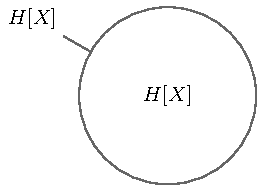
\includegraphics{../appendix2/figures/tikz/1var/1var_bare}
\caption{The simplest I-diagram - one random variable, $X$.}
\label{fig:1var_bare}
\end{figure}

\begin{figure}[h]
\centering
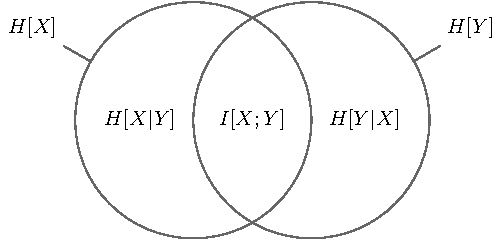
\includegraphics{../appendix2/figures/tikz/2var/2var_bare}
\caption{I-diagram for two random variables, $X$ and $Y$.}
\label{fig:2var_bare}
\end{figure}

In an I-diagram involving two random variables, the area of intersection of two random variable shapes, $X, Y$, corresponds to the mutual information between those random variables, $I[X;Y]$ (see Fig.~\ref{fig:2var_IXY}). This is the information that the two random variables share.

\begin{figure}[h]
\centering
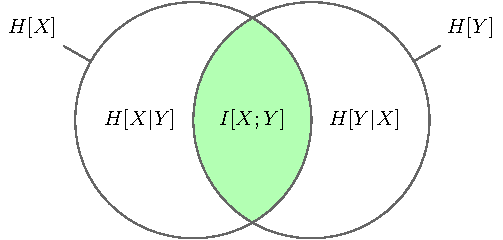
\includegraphics{../appendix2/figures/tikz/2var/2var_IXY}
\caption{The mutual information between $X$ and $Y$ is highlighted.}
\label{fig:2var_IXY}
\end{figure}

The area of random variable $X$ that is unoccluded by random variable $Y$ corresponds to the conditional entropy, $H[X|Y]$. This is the uncertainty in $X$ that remains when $Y$ is known.

\begin{figure}[h]
\centering
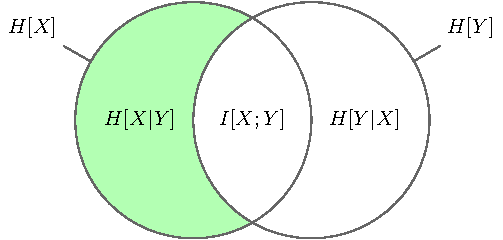
\includegraphics{../appendix2/figures/tikz/2var/2var_HX_Y}
\caption{The conditional entropy of $X$ given $Y$ is highlighted.}
\label{fig:2var_HX_Y}
\end{figure}

Now consider a three variable I-diagram. What is the uncertainty in $X$ given \emph{both} $Y$ and $Z$? This is notated $H[X|YZ]$ as in Fig.~\ref{fig:3var_HX_YZ}.

\begin{figure}[h]
\centering
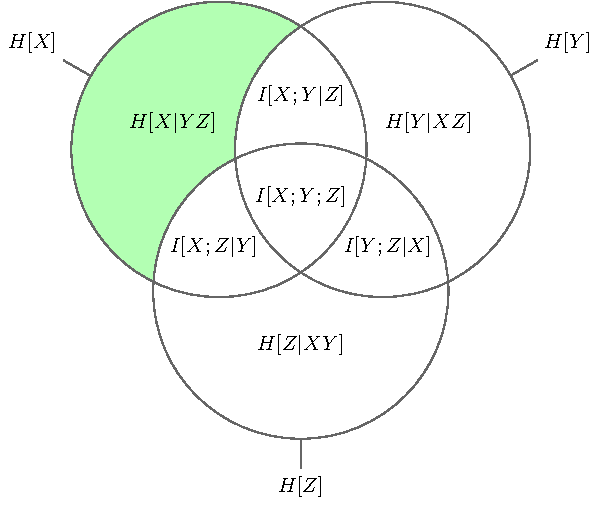
\includegraphics{../appendix2/figures/tikz/3var/3var_HX_YZ}
\caption{The conditional entropy of $X$ given $Y$ and $Z$ is highlighted.}
\label{fig:3var_HX_YZ}
\end{figure}

 We can equivalently think of merging $Y$ and $Z$ to form a random variable, $W$, with a larger event space. In this light, our quantity of interest would look like $H[X|W]$. We can think of this graphically quite naturally by considering $W$ as the union of $Y$ and $Z$ (see Fig.~\ref{fig:3var_HX_W}).

\begin{figure}[h]
\centering
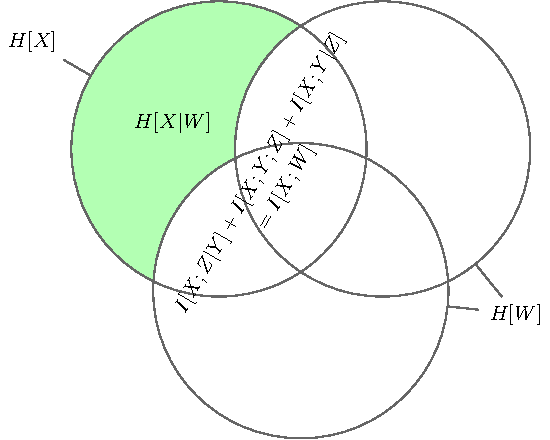
\includegraphics{../appendix2/figures/tikz/3var/3var_HX_W}
\caption{The mutual information of $X$ and joint variable $W$ is highlighted.}
\label{fig:3var_HX_W}
\end{figure}

Now considering a three variable I-diagram, the area of intersection between $X$ and $Y$ that is unoccluded by $Z$ is the conditional mutual information, $I[X;Y|Z]$ (see Fig.~\ref{fig:3var_IXY_Z}). This is the information shared by $X$ and $Y$ when $Z$ is known. Adding knowledge about $Z$ can either increase or decrease the (conditioned) mutual information.

From these diagrams, e.g. Fig.~\ref{fig:2var_bare}, we can visually prove such identities as:
\begin{align*}
H[X Y] &= H[X|Y] + I[X;Y] + H[Y|X]\\
I[X;Y] &= H[X] - H[X|Y]
\end{align*}

\begin{figure}[h]
\centering
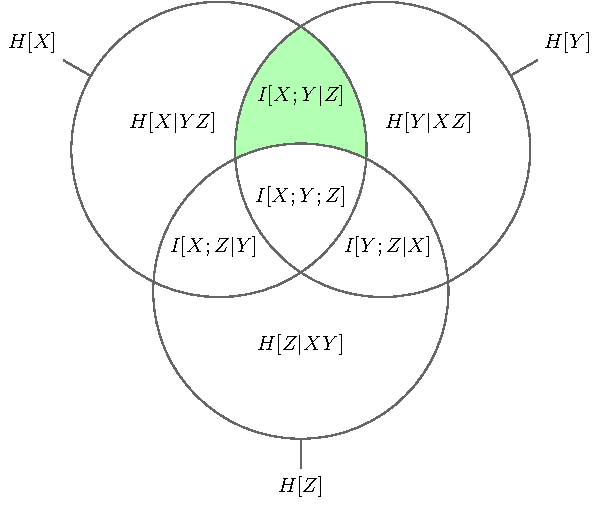
\includegraphics{../appendix2/figures/tikz/3var/3var_IXY_Z}
\caption{The conditional mutual entropy of $X$ and $Y$ given $Z$ is highlighted.}
\label{fig:3var_IXY_Z}
\end{figure}

\subsection{Stratification of a Composite Variable}
Just as more than one random variable can be considered as a composite variable, as in Fig.~\ref{fig:3var_HX_W}, a composite variable can be stratified in a very intuitive way. Consider the set of random variables $\{\MeasSymbol_0, \MeasSymbol_1, \MeasSymbol_2, \MeasSymbol_3, \MeasSymbol_4\}$. The composite random variable $\MeasSymbol_0^5$ can be stratified by the set $\{\MeasSymbol_{0}^{1}, \MeasSymbol_{0}^{2}, \MeasSymbol_{0}^{3}, \MeasSymbol_{0}^{4}, \MeasSymbol_{0}^{5}\}$. These results are generic for any set of `stratifying' variables.

\begin{Def}
Given a set $\mathbf{X} = \{X_1, \ldots, X_N\}$ for some integer, $N$, a set of subsets of $\mathbf{X}$, $\mathbf{Y}$, is called \emph{stratifying} if a total ordering on $\mathbf{Y}$ is induced by the relation $\subset$.
\end{Def}

For any such $\mathbf{X}$, we have the stratifying set $\mathbf{Y} = \{\{X_1\}, \{X_1, X_2\}, \ldots, \{X_1, X_2, \ldots, X_N\}\}$.

We can stratify the past random variables of a process as in Fig.~\ref{fig:FoliationPast}.

\begin{figure}[h]
\centering
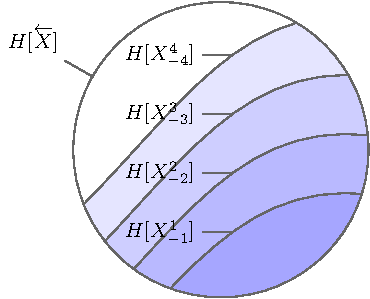
\includegraphics{../appendix2/figures/tikz/FoliationPast}
\caption{The standard stratification of the conglomerate random variable $\protect \Past$.}
\label{fig:FoliationPast}
\end{figure}

That this is true follows straightforwardly from the duality between information measures and set operations demonstrated by \FIX{cite Yeung}.

Additionally, the I-diagram involving a stratified variable and one additional variable has the form in Fig.~\ref{fig:FolationPastAndZ}. To see that this is not a trivial statement, consider the following scenario. Let random variables $X$ and $Y$ each be fair coins. Then let $Z$ be the exclusive-or (XOR) of $X$ and $Y$.  If we were to begin with the I-diagram for just $X$ and $Y$, we would have the following picture.
\FIX{graphic here}

Then naively `adding' $Z$ to the I-diagram yields the following picture.
\FIX{graphic here}

This fails to capture the true information theoretic structure. Specifically, it does not capture that $I[X;Y|Z]=1$ or that $I[X;Y;Z]=-1$. The correct picture does not allow for regions to be eliminated before the addition of all variables to the diagram. This is why it is non-trivial to `naturally' add $Z$ to the stratified variable I-diagram.
 


\ifx\master\undefined% AUTOCOMPILE
% Allows for individual chapters to be compiled.

% Usage:
% \ifx\master\undefined% AUTOCOMPILE
% Allows for individual chapters to be compiled.

% Usage:
% \ifx\master\undefined% AUTOCOMPILE
% Allows for individual chapters to be compiled.

% Usage:
% \ifx\master\undefined\input{../settings/autocompile}\fi
% (place at start and end of chapter file)

\ifx\noprelim\undefined
    % first time included
    % input preamble files
    \input{../settings/phdsetup}

    \begin{document}
    \def\noprelim{}
\else
    % already included once
    % input post files

    \singlespacing
    \bibliographystyle{../bibliography/expanded}
    \bibliography{../bibliography/references}

    \end{document}
\fi\fi
% (place at start and end of chapter file)

\ifx\noprelim\undefined
    % first time included
    % input preamble files
    % [ USER VARIABLES ]

\def\PHDTITLE {Extensions of the Theory of Computational Mechanics}
\def\PHDAUTHOR{Evan Klose Friis}
\def\PHDSCHOOL{University of California, Davis}

\def\PHDMONTH {June}
\def\PHDYEAR  {2011}
\def\PHDDEPT {Physics}

\def\BSSCHOOL {University of California at San Diego}
\def\BSYEAR   {2005}

\def\PHDCOMMITTEEA{Professor John Conway}
\def\PHDCOMMITTEEB{Professor Robin Erbacher}
\def\PHDCOMMITTEEC{Professor Mani Tripathi}

% [ GLOBAL SETUP ]

\documentclass[letterpaper,oneside,11pt]{report}

\usepackage{calc}
\usepackage{breakcites}
\usepackage[newcommands]{ragged2e}

\usepackage[pdftex]{graphicx}
\usepackage{epstopdf}

%\usepackage{tikz}
%\usetikzlibrary{positioning} % [right=of ...]
%\usetikzlibrary{fit} % [fit= ...]

%\pgfdeclarelayer{background layer}
%\pgfdeclarelayer{foreground layer}
%\pgfsetlayers{background layer,main,foreground layer}

%\newenvironment{wrap}{\noindent\begin{minipage}[t]{\linewidth}\vspace{-0.5\normalbaselineskip}\centering}{\vspace{0.5\normalbaselineskip}\end{minipage}}

%% [Venn diagram environment]
%\newenvironment{venn2}
%{\begin{tikzpicture} [every pin/.style={text=black, text opacity=1.0, pin distance=0.5cm, pin edge={black!60, semithick}},
%% define a new style 'venn'
%venn/.style={circle, draw=black!60, semithick, minimum size = 4cm}]
%
%% create circle and give it external (pin) label
%\node[venn] (X) at (-1,0) [pin={150:$H[X]$}] {};
%\node[venn] (Y) at (1,0) [pin={30:$H[Y]$}] {};
%
%% place labels of the atoms by hand
%\node at (-1.9,0) {$H[X|Y]$};
%\node at (1.9,0) {$H[Y|X]$};
%\node at (0,0) {$I[X;Y]$};}
%{\end{tikzpicture}}

%\newcommand{\wrapmath}[1]{\begin{wrap}\begin{tikzpicture}[every node/.style={inner ysep=0ex, inner xsep=0em}]\node[] {$\displaystyle\begin{aligned} #1\end{aligned}$};\end{tikzpicture}\end{wrap}}

\renewenvironment{abstract}{\chapter*{Abstract}}{}
\renewcommand{\bibname}{Bibliography}
\renewcommand{\contentsname}{Table of Contents}

\makeatletter
\renewcommand{\@biblabel}[1]{\textsc{#1}}
\makeatother

% [ FONT SETTINGS ]

\usepackage[tbtags, intlimits, namelimits]{amsmath}
\usepackage[adobe-utopia]{mathdesign}

\DeclareSymbolFont{pazomath}{OMS}{zplm}{m}{n}
\DeclareSymbolFontAlphabet{\mathcal}{pazomath}
\SetMathAlphabet\mathcal{bold}{OMS}{zplm}{b}{n}

\SetSymbolFont{largesymbols}{normal}{OMX}{zplm}{m}{n}
\SetSymbolFont{largesymbols}{bold}{OMX}{zplm}{m}{n}
\SetSymbolFont{symbols}{normal}{OMS}{zplm}{m}{n}
\SetSymbolFont{symbols}{bold}{OMS}{zplm}{b}{n}

\renewcommand{\sfdefault}{phv}
\renewcommand{\ttdefault}{fvm}

\widowpenalty 8000
\clubpenalty  8000

% [ PAGE LAYOUT ]
\usepackage{geometry}
\geometry{lmargin = 1.5in}
\geometry{rmargin = 1.0in}
\geometry{tmargin = 1.0in}
\geometry{bmargin = 1.0in}

% [ PDF SETTINGS ]

\usepackage[final]{hyperref}
\hypersetup{breaklinks  = true}
\hypersetup{colorlinks  = true}
\hypersetup{linktocpage = false}
\hypersetup{linkcolor   = blue}
\hypersetup{citecolor   = green}
\hypersetup{urlcolor    = black}
\hypersetup{plainpages  = false}
\hypersetup{pageanchor  = true}
\hypersetup{pdfauthor   = {\PHDAUTHOR}}
\hypersetup{pdftitle    = {\PHDTITLE}}
\hypersetup{pdfsubject  = {Dissertation, \PHDSCHOOL}}
\urlstyle{same}

% [ LETTER SPACING ]

\usepackage[final]{microtype}
\microtypesetup{protrusion=compatibility}
\microtypesetup{expansion=false}

\newcommand{\upper}[1]{\MakeUppercase{#1}}
\let\lsscshape\scshape

\ifcase\pdfoutput\else\microtypesetup{letterspace=15}
\renewcommand{\scshape}{\lsscshape\lsstyle}
\renewcommand{\upper}[1]{\textls[50]{\MakeUppercase{#1}}}\fi

% [ LINE SPACING ]

\usepackage[doublespacing]{setspace}
\renewcommand{\displayskipstretch}{0.0}

\setlength{\parskip   }{0em}
\setlength{\parindent }{2em}

% [ TABLE FORMATTING ]

\usepackage{booktabs}
\setlength{\heavyrulewidth}{1.5\arrayrulewidth}
\setlength{\lightrulewidth}{1.0\arrayrulewidth}
\setlength{\doublerulesep }{2.0\arrayrulewidth}

% [ SECTION FORMATTING ]

\usepackage[largestsep,nobottomtitles*]{titlesec}
\renewcommand{\bottomtitlespace}{0.75in}

\titleformat{\chapter}[display]{\bfseries\huge\singlespacing}{\filleft\textsc{\LARGE \chaptertitlename\ \thechapter}}{-0.2ex}{\titlerule[3pt]\vspace{0.2ex}}[]

\titleformat{\section}{\LARGE}{\S\thesection\hspace{0.5em}}{0ex}{}
\titleformat{\subsection}{\Large}{\S\thesubsection\hspace{0.5em}}{0ex}{}
\titleformat{\subsubsection}{\large}{\thesubsubsection\hspace{0.5em}}{0ex}{}

\titlespacing*{\chapter}{0em}{6ex}{4ex plus 2ex minus 0ex}
\titlespacing*{\section}{0em}{2ex plus 3ex minus 1ex}{0.5ex plus 0.5ex minus 0.5ex}
\titlespacing*{\subsection}{0ex}{2ex plus 3ex minus 1ex}{0ex}
\titlespacing*{\subsubsection}{0ex}{2ex plus 0ex minus 1ex}{0ex}

% [ HEADER SETTINGS ]

\usepackage{fancyhdr}

\setlength{\headheight}{\normalbaselineskip}
\setlength{\footskip  }{0.5in}
\setlength{\headsep   }{0.5in-\headheight}

\fancyheadoffset[R]{0.5in}
\renewcommand{\headrulewidth}{0pt}
\renewcommand{\footrulewidth}{0pt}

\newcommand{\pagebox}{\parbox[r][\headheight][t]{0.5in}{\hspace\fill\thepage}}

\newcommand{\prelimheaders}{\ifx\prelim\undefined\renewcommand{\thepage}{\textit{\roman{page}}}\fancypagestyle{plain}{\fancyhf{}\fancyfoot[L]{\makebox[\textwidth-0.5in]{\thepage}}}\pagestyle{plain}\def\prelim{}\fi}

\newcommand{\normalheaders}{\renewcommand{\thepage}{\arabic{page}}\fancypagestyle{plain}{\fancyhf{}\fancyhead[R]{\pagebox}}\pagestyle{plain}}

\normalheaders{}

% [ CUSTOM COMMANDS ]

\newcommand{\signaturebox}[1]{\multicolumn{1}{p{4in}}{\vspace{3ex}}\\\midrule #1\\}

%\input{../includes/cmechabbrev}

% [some math stuff - maybe stick in sep file]
\usepackage{amsthm}
\usepackage{amscd}
\theoremstyle{plain}    \newtheorem{Lem}{Lemma}
\theoremstyle{plain}    \newtheorem*{ProLem}{Proof}
\theoremstyle{plain} 	\newtheorem{Cor}{Corollary}
\theoremstyle{plain} 	\newtheorem*{ProCor}{Proof}
\theoremstyle{plain} 	\newtheorem{The}{Theorem}
\theoremstyle{plain} 	\newtheorem*{ProThe}{Proof}
\theoremstyle{plain} 	\newtheorem{Prop}{Proposition}
\theoremstyle{plain} 	\newtheorem*{ProProp}{Proof}
\theoremstyle{plain} 	\newtheorem*{Conj}{Conjecture}
\theoremstyle{plain}	\newtheorem*{Rem}{Remark}
\theoremstyle{plain}	\newtheorem*{Def}{Definition} 
\theoremstyle{plain}	\newtheorem*{Not}{Notation}

% [uniform figure scaling - maybe this is not a good idea]
\def\figscale{.7}
\def\lscale{1.0}

% [FIX ME! - red makes it easier to spot]
\newcommand{\FIX}[1]{\textbf{\textcolor{red}{#1}}}


    \begin{document}
    \def\noprelim{}
\else
    % already included once
    % input post files

    \singlespacing
    \bibliographystyle{../bibliography/expanded}
    \bibliography{../bibliography/references}

    \end{document}
\fi\fi
% (place at start and end of chapter file)

\ifx\noprelim\undefined
    % first time included
    % input preamble files
    % [ USER VARIABLES ]

\def\PHDTITLE {Extensions of the Theory of Computational Mechanics}
\def\PHDAUTHOR{Evan Klose Friis}
\def\PHDSCHOOL{University of California, Davis}

\def\PHDMONTH {June}
\def\PHDYEAR  {2011}
\def\PHDDEPT {Physics}

\def\BSSCHOOL {University of California at San Diego}
\def\BSYEAR   {2005}

\def\PHDCOMMITTEEA{Professor John Conway}
\def\PHDCOMMITTEEB{Professor Robin Erbacher}
\def\PHDCOMMITTEEC{Professor Mani Tripathi}

% [ GLOBAL SETUP ]

\documentclass[letterpaper,oneside,11pt]{report}

\usepackage{calc}
\usepackage{breakcites}
\usepackage[newcommands]{ragged2e}

\usepackage[pdftex]{graphicx}
\usepackage{epstopdf}

%\usepackage{tikz}
%\usetikzlibrary{positioning} % [right=of ...]
%\usetikzlibrary{fit} % [fit= ...]

%\pgfdeclarelayer{background layer}
%\pgfdeclarelayer{foreground layer}
%\pgfsetlayers{background layer,main,foreground layer}

%\newenvironment{wrap}{\noindent\begin{minipage}[t]{\linewidth}\vspace{-0.5\normalbaselineskip}\centering}{\vspace{0.5\normalbaselineskip}\end{minipage}}

%% [Venn diagram environment]
%\newenvironment{venn2}
%{\begin{tikzpicture} [every pin/.style={text=black, text opacity=1.0, pin distance=0.5cm, pin edge={black!60, semithick}},
%% define a new style 'venn'
%venn/.style={circle, draw=black!60, semithick, minimum size = 4cm}]
%
%% create circle and give it external (pin) label
%\node[venn] (X) at (-1,0) [pin={150:$H[X]$}] {};
%\node[venn] (Y) at (1,0) [pin={30:$H[Y]$}] {};
%
%% place labels of the atoms by hand
%\node at (-1.9,0) {$H[X|Y]$};
%\node at (1.9,0) {$H[Y|X]$};
%\node at (0,0) {$I[X;Y]$};}
%{\end{tikzpicture}}

%\newcommand{\wrapmath}[1]{\begin{wrap}\begin{tikzpicture}[every node/.style={inner ysep=0ex, inner xsep=0em}]\node[] {$\displaystyle\begin{aligned} #1\end{aligned}$};\end{tikzpicture}\end{wrap}}

\renewenvironment{abstract}{\chapter*{Abstract}}{}
\renewcommand{\bibname}{Bibliography}
\renewcommand{\contentsname}{Table of Contents}

\makeatletter
\renewcommand{\@biblabel}[1]{\textsc{#1}}
\makeatother

% [ FONT SETTINGS ]

\usepackage[tbtags, intlimits, namelimits]{amsmath}
\usepackage[adobe-utopia]{mathdesign}

\DeclareSymbolFont{pazomath}{OMS}{zplm}{m}{n}
\DeclareSymbolFontAlphabet{\mathcal}{pazomath}
\SetMathAlphabet\mathcal{bold}{OMS}{zplm}{b}{n}

\SetSymbolFont{largesymbols}{normal}{OMX}{zplm}{m}{n}
\SetSymbolFont{largesymbols}{bold}{OMX}{zplm}{m}{n}
\SetSymbolFont{symbols}{normal}{OMS}{zplm}{m}{n}
\SetSymbolFont{symbols}{bold}{OMS}{zplm}{b}{n}

\renewcommand{\sfdefault}{phv}
\renewcommand{\ttdefault}{fvm}

\widowpenalty 8000
\clubpenalty  8000

% [ PAGE LAYOUT ]
\usepackage{geometry}
\geometry{lmargin = 1.5in}
\geometry{rmargin = 1.0in}
\geometry{tmargin = 1.0in}
\geometry{bmargin = 1.0in}

% [ PDF SETTINGS ]

\usepackage[final]{hyperref}
\hypersetup{breaklinks  = true}
\hypersetup{colorlinks  = true}
\hypersetup{linktocpage = false}
\hypersetup{linkcolor   = blue}
\hypersetup{citecolor   = green}
\hypersetup{urlcolor    = black}
\hypersetup{plainpages  = false}
\hypersetup{pageanchor  = true}
\hypersetup{pdfauthor   = {\PHDAUTHOR}}
\hypersetup{pdftitle    = {\PHDTITLE}}
\hypersetup{pdfsubject  = {Dissertation, \PHDSCHOOL}}
\urlstyle{same}

% [ LETTER SPACING ]

\usepackage[final]{microtype}
\microtypesetup{protrusion=compatibility}
\microtypesetup{expansion=false}

\newcommand{\upper}[1]{\MakeUppercase{#1}}
\let\lsscshape\scshape

\ifcase\pdfoutput\else\microtypesetup{letterspace=15}
\renewcommand{\scshape}{\lsscshape\lsstyle}
\renewcommand{\upper}[1]{\textls[50]{\MakeUppercase{#1}}}\fi

% [ LINE SPACING ]

\usepackage[doublespacing]{setspace}
\renewcommand{\displayskipstretch}{0.0}

\setlength{\parskip   }{0em}
\setlength{\parindent }{2em}

% [ TABLE FORMATTING ]

\usepackage{booktabs}
\setlength{\heavyrulewidth}{1.5\arrayrulewidth}
\setlength{\lightrulewidth}{1.0\arrayrulewidth}
\setlength{\doublerulesep }{2.0\arrayrulewidth}

% [ SECTION FORMATTING ]

\usepackage[largestsep,nobottomtitles*]{titlesec}
\renewcommand{\bottomtitlespace}{0.75in}

\titleformat{\chapter}[display]{\bfseries\huge\singlespacing}{\filleft\textsc{\LARGE \chaptertitlename\ \thechapter}}{-0.2ex}{\titlerule[3pt]\vspace{0.2ex}}[]

\titleformat{\section}{\LARGE}{\S\thesection\hspace{0.5em}}{0ex}{}
\titleformat{\subsection}{\Large}{\S\thesubsection\hspace{0.5em}}{0ex}{}
\titleformat{\subsubsection}{\large}{\thesubsubsection\hspace{0.5em}}{0ex}{}

\titlespacing*{\chapter}{0em}{6ex}{4ex plus 2ex minus 0ex}
\titlespacing*{\section}{0em}{2ex plus 3ex minus 1ex}{0.5ex plus 0.5ex minus 0.5ex}
\titlespacing*{\subsection}{0ex}{2ex plus 3ex minus 1ex}{0ex}
\titlespacing*{\subsubsection}{0ex}{2ex plus 0ex minus 1ex}{0ex}

% [ HEADER SETTINGS ]

\usepackage{fancyhdr}

\setlength{\headheight}{\normalbaselineskip}
\setlength{\footskip  }{0.5in}
\setlength{\headsep   }{0.5in-\headheight}

\fancyheadoffset[R]{0.5in}
\renewcommand{\headrulewidth}{0pt}
\renewcommand{\footrulewidth}{0pt}

\newcommand{\pagebox}{\parbox[r][\headheight][t]{0.5in}{\hspace\fill\thepage}}

\newcommand{\prelimheaders}{\ifx\prelim\undefined\renewcommand{\thepage}{\textit{\roman{page}}}\fancypagestyle{plain}{\fancyhf{}\fancyfoot[L]{\makebox[\textwidth-0.5in]{\thepage}}}\pagestyle{plain}\def\prelim{}\fi}

\newcommand{\normalheaders}{\renewcommand{\thepage}{\arabic{page}}\fancypagestyle{plain}{\fancyhf{}\fancyhead[R]{\pagebox}}\pagestyle{plain}}

\normalheaders{}

% [ CUSTOM COMMANDS ]

\newcommand{\signaturebox}[1]{\multicolumn{1}{p{4in}}{\vspace{3ex}}\\\midrule #1\\}

%%%% macros fro standard references
%\eqref provided by amsmath
\newcommand{\figref}[1]{Fig.~\ref{#1}}
\newcommand{\tableref}[1]{Table~\ref{#1}}
\newcommand{\refcite}[1]{Ref.~\cite{#1}}

% Abbreviations from CMPPSS:

\newcommand{\eM}     {\mbox{$\epsilon$-machine}}
\newcommand{\eMs}    {\mbox{$\epsilon$-machines}}
\newcommand{\EM}     {\mbox{$\epsilon$-Machine}}
\newcommand{\EMs}    {\mbox{$\epsilon$-Machines}}
\newcommand{\eT}     {\mbox{$\epsilon$-transducer}}
\newcommand{\eTs}    {\mbox{$\epsilon$-transducers}}
\newcommand{\ET}     {\mbox{$\epsilon$-Transducer}}
\newcommand{\ETs}    {\mbox{$\epsilon$-Transducers}}

% Processes and sequences

\newcommand{\Process}{\mathcal{P}}

\newcommand{\ProbMach}{\Prob_{\mathrm{M}}}
\newcommand{\Lmax}   { {L_{\mathrm{max}}}}
\newcommand{\MeasAlphabet}	{\mathcal{A}}
% Original
%\newcommand{\MeasSymbol}   { {S} }
%\newcommand{\meassymbol}   { {s} }
% New symbol
\newcommand{\MeasSymbol}   { {X} }
\newcommand{\meassymbol}   { {x} }
\newcommand{\BiInfinity}	{ \overleftrightarrow {\MeasSymbol} }
\newcommand{\biinfinity}	{ \overleftrightarrow {\meassymbol} }
\newcommand{\Past}	{ \overleftarrow {\MeasSymbol} }
\newcommand{\past}	{ {\overleftarrow {\meassymbol}} }
\newcommand{\pastprime}	{ {\past}^{\prime}}
\newcommand{\Future}	{ \overrightarrow{\MeasSymbol} }
\newcommand{\future}	{ \overrightarrow{\meassymbol} }
\newcommand{\futureprime}	{ {\future}^{\prime}}
\newcommand{\PastPrime}	{ {\Past}^{\prime}}
\newcommand{\FuturePrime}	{ {\overrightarrow{\meassymbol}}^\prime }
\newcommand{\PastDblPrime}	{ {\overleftarrow{\meassymbol}}^{\prime\prime} }
\newcommand{\FutureDblPrime}	{ {\overrightarrow{\meassymbol}}^{\prime\prime} }
\newcommand{\pastL}	{ {\overleftarrow {\meassymbol}}{}^L }
\newcommand{\PastL}	{ {\overleftarrow {\MeasSymbol}}{}^L }
\newcommand{\PastLt}	{ {\overleftarrow {\MeasSymbol}}_t^L }
\newcommand{\PastLLessOne}	{ {\overleftarrow {\MeasSymbol}}^{L-1} }
\newcommand{\futureL}	{ {\overrightarrow{\meassymbol}}{}^L }
\newcommand{\FutureL}	{ {\overrightarrow{\MeasSymbol}}{}^L }
\newcommand{\FutureLt}	{ {\overrightarrow{\MeasSymbol}}_t^L }
\newcommand{\FutureLLessOne}	{ {\overrightarrow{\MeasSymbol}}^{L-1} }
\newcommand{\pastLprime}	{ {\overleftarrow {\meassymbol}}^{L^\prime} }
\newcommand{\futureLprime}	{ {\overrightarrow{\meassymbol}}^{L^\prime} }
\newcommand{\AllPasts}	{ { \overleftarrow {\rm {\bf \MeasSymbol}} } }
\newcommand{\AllFutures}	{ \overrightarrow {\rm {\bf \MeasSymbol}} }
\newcommand{\FutureSet}	{ \overrightarrow{\bf \MeasSymbol}}

% Causal states and epsilon-machines
\newcommand{\CausalState}	{ \mathcal{S} }
\newcommand{\CausalStatePrime}	{ {\CausalState}^{\prime}}
\newcommand{\causalstate}	{ \sigma }
\newcommand{\CausalStateSet}	{ \boldsymbol{\CausalState} }
\newcommand{\AlternateState}	{ \mathcal{R} }
\newcommand{\AlternateStatePrime}	{ {\cal R}^{\prime} }
\newcommand{\alternatestate}	{ \rho }
\newcommand{\alternatestateprime}	{ {\rho^{\prime}} }
\newcommand{\AlternateStateSet}	{ \boldsymbol{\AlternateState} }
\newcommand{\PrescientState}	{ \widehat{\AlternateState} }
\newcommand{\prescientstate}	{ \widehat{\alternatestate} }
\newcommand{\PrescientStateSet}	{ \boldsymbol{\PrescientState}}
\newcommand{\CausalEquivalence}	{ {\sim}_{\epsilon} }
\newcommand{\CausalEquivalenceNot}	{ {\not \sim}_{\epsilon}}

\newcommand{\NonCausalEquivalence}	{ {\sim}_{\eta} }
\newcommand{\NextObservable}	{ {\overrightarrow {\MeasSymbol}}^1 }
\newcommand{\LastObservable}	{ {\overleftarrow {\MeasSymbol}}^1 }
%\newcommand{\Prob}		{ {\rm P}}
\newcommand{\Prob}      {\Pr} % use standard command
\newcommand{\ProbAnd}	{ {,\;} }
\newcommand{\LLimit}	{ {L \rightarrow \infty}}
\newcommand{\Cmu}		{C_\mu}
\newcommand{\hmu}		{h_\mu}
\newcommand{\EE}		{{\bf E}}
\newcommand{\Measurable}{{\bf \mu}}

% Process Crypticity
\newcommand{\PC}		{\chi}
\newcommand{\FuturePC}		{\PC^+}
\newcommand{\PastPC}		{\PC^-}
% Causal Irreversibility
\newcommand{\CI}		{\Xi}
\newcommand{\ReverseMap}	{r}
\newcommand{\ForwardMap}	{f}

% Abbreviations from IB:
% None that aren't already in CMPPSS

% Abbreviations from Extensive Estimation:
\newcommand{\EstCausalState}	{\widehat{\CausalState}}
\newcommand{\estcausalstate}	{\widehat{\causalstate}}
\newcommand{\EstCausalStateSet}	{\boldsymbol{\EstCausalState}}
\newcommand{\EstCausalFunc}	{\widehat{\epsilon}}
\newcommand{\EstCmu}		{\widehat{\Cmu}}
\newcommand{\PastLOne}	{{\Past}^{L+1}}
\newcommand{\pastLOne}	{{\past}^{L+1}}

% Abbreviations from $\epsilon$-Transducers:
\newcommand{\InAlphabet}	{ \mathcal{A}}
\newcommand{\insymbol}		{ a}
\newcommand{\OutAlphabet}	{ \mathcal{B}}
\newcommand{\outsymbol}		{ b}
\newcommand{\InputSimple}	{ X}
\newcommand{\inputsimple}	{ x}
\newcommand{\BottleneckVar}	{\tilde{\InputSimple}}
\newcommand{\bottleneckvar}	{\tilde{\inputsimple}}
\newcommand{\InputSpace}	{ \mathbf{\InputSimple}}
\newcommand{\InputBi}	{ \overleftrightarrow {\InputSimple} }
\newcommand{\inputbi}	{ \overleftrightarrow {\inputsimple} }
\newcommand{\InputPast}	{ \overleftarrow {\InputSimple} }
\newcommand{\inputpast}	{ \overleftarrow {\inputsimple} }
\newcommand{\InputFuture}	{ \overrightarrow {\InputSimple} }
\newcommand{\inputfuture}	{ \overrightarrow {\inputsimple} }
\newcommand{\NextInput}	{ {{\InputFuture}^{1}}}
\newcommand{\NextOutput}	{ {\OutputFuture}^{1}}
\newcommand{\OutputSimple}	{ Y}
\newcommand{\outputsimple}	{ y}
\newcommand{\OutputSpace}	{ \mathbf{\OutputSimple}}
\newcommand{\OutputBi}	{ \overleftrightarrow{\OutputSimple} }
\newcommand{\outputbi}	{ \overleftrightarrow{\outputsimple} }
\newcommand{\OutputPast}	{ \overleftarrow{\OutputSimple} }
\newcommand{\outputpast}	{ \overleftarrow{\outputsimple} }
\newcommand{\OutputFuture}	{ \overrightarrow{\OutputSimple} }
\newcommand{\outputfuture}	{ \overrightarrow{\outputsimple} }
\newcommand{\OutputL}	{ {\OutputFuture}^L}
\newcommand{\outputL}	{ {\outputfuture}^L}
\newcommand{\InputLLessOne}	{ {\InputFuture}^{L-1}}
\newcommand{\inputLlessone}	{ {\inputufutre}^{L-1}}
\newcommand{\OutputPastLLessOne}	{{\OutputPast}^{L-1}_{-1}}
\newcommand{\outputpastLlessone}	{{\outputpast}^{L-1}}
\newcommand{\OutputPastLessOne}	{{\OutputPast}_{-1}}
\newcommand{\outputpastlessone}	{{\outputpast}_{-1}}
\newcommand{\OutputPastL}	{{\OutputPast}^{L}}
\newcommand{\OutputLPlusOne}	{ {\OutputFuture}^{L+1}}
\newcommand{\outputLplusone}	{ {\outputfutre}^{L+1}}
\newcommand{\InputPastL}	{{\InputPast}^{L}}
\newcommand{\inputpastL}	{{\inputpast}^{L}}
\newcommand{\JointPast}	{{(\InputPast,\OutputPast)}}
\newcommand{\jointpast}	{{(\inputpast,\outputpast)}}
\newcommand{\jointpastone}	{{(\inputpast_1,\outputpast_1)}}
\newcommand{\jointpasttwo}	{{(\inputpast_2,\outputpast_2)}}
\newcommand{\jointpastprime} {{({\inputpast}^{\prime},{\outputpast}^{\prime})}}
\newcommand{\NextJoint}	{{(\NextInput,\NextOutput)}}
\newcommand{\nextjoint}	{{(\insymbol,\outsymbol)}}
\newcommand{\AllInputPasts}	{ { \overleftarrow {\rm \InputSpace}}}
\newcommand{\AllOutputPasts}	{ {\overleftarrow {\rm \OutputSpace}}}
\newcommand{\DetCausalState}	{ {{\cal S}_D }}
\newcommand{\detcausalstate}	{ {{\sigma}_D} }
\newcommand{\DetCausalStateSet}	{ \boldsymbol{{\CausalState}_D}}
\newcommand{\DetCausalEquivalence}	{ {\sim}_{{\epsilon}_{D}}}
\newcommand{\PrescientEquivalence}	{ {\sim}_{\widehat{\eta}}}
\newcommand{\FeedbackCausalState}	{ \mathcal{F}}
\newcommand{\feedbackcausalstate}	{ \phi}
\newcommand{\FeedbackCausalStateSet}	{ \mathbf{\FeedbackCausalState}}
\newcommand{\JointCausalState}		{ \mathcal{J}}
\newcommand{\JointCausalStateSet}	{ \mathbf{\JointCausalState}}
\newcommand{\UtilityFunctional}	{ {\mathcal{L}}}
\newcommand{\NatureState}	{ {\Omega}}
\newcommand{\naturestate}	{ {\omega}}
\newcommand{\NatureStateSpace}	{ {\mathbf{\NatureState}}}
\newcommand{\AnAction}	{ {A}}
\newcommand{\anaction}	{ {a}}
\newcommand{\ActionSpace}	{ {\mathbf{\AnAction}}}

% Abbreviations from RURO:
\newcommand{\InfoGain}[2] { \mathcal{D} \left( {#1} || {#2} \right) }

% Abbreviations from Upper Bound:
\newcommand{\lcm}	{{\rm lcm}}
% Double-check that this isn't in the math set already!

% Abbreviations from Emergence in Space
\newcommand{\ProcessAlphabet}	{\MeasAlphabet}
\newcommand{\ProbEst}			{ {\widehat{\Prob}_N}}
\newcommand{\STRegion}			{ {\mathrm K}}
\newcommand{\STRegionVariable}		{ K}
\newcommand{\stregionvariable}		{ k}
\newcommand{\GlobalPast}		{ \overleftarrow{G}} 
\newcommand{\globalpast}		{ \overleftarrow{g}} 
\newcommand{\GlobalFuture}		{ \overrightarrow{G}}
\newcommand{\globalfuture}		{ \overrightarrow{g}}
\newcommand{\GlobalState}		{ \mathcal{G}}
\newcommand{\globalstate}		{ \gamma}
\newcommand{\GlobalStateSet}		{ {\mathbf \GlobalState}}
\newcommand{\LocalPast}			{ \overleftarrow{L}} 
\newcommand{\localpast}			{ \overleftarrow{l}}
\newcommand{\AllLocalPasts}		{ \mathbf{\LocalPast}}
\newcommand{\LocalPastRegion}		{ \overleftarrow{\mathrm L}}
\newcommand{\LocalFuture}		{ \overrightarrow{L}}
\newcommand{\localfuture}		{ \overrightarrow{l}}
\newcommand{\LocalFutureRegion}		{ \overrightarrow{\mathrm L}}
\newcommand{\LocalState}		{ \mathcal{L}}
\newcommand{\localstate}		{ \lambda}
\newcommand{\LocalStateSet}		{ {\mathbf \LocalState}}
\newcommand{\PatchPast}			{ \overleftarrow{P}}
\newcommand{\patchpast}			{ \overleftarrow{p}}
\newcommand{\PatchPastRegion}		{ \overleftarrow{\mathrm P}}
\newcommand{\PatchFuture}		{ \overrightarrow{P}}
\newcommand{\patchfuture}		{ \overrightarrow{p}}
\newcommand{\PatchFutureRegion}		{ \overrightarrow{\mathrm P}}
\newcommand{\PatchState}		{ \mathcal{P}}
\newcommand{\patchstate}		{ \pi}
\newcommand{\PatchStateSet}		{ {\mathbf \PatchState}}
\newcommand{\LocalStatesInPatch}	{\vec{\LocalState}}
\newcommand{\localstatesinpatch}	{\vec{\localstate}}
\newcommand{\PointInstantX}		{ {\mathbf x}}
% Galles's original LaTeX for the cond. indep. symbol follows:
\newcommand{\compos}{\mbox{$~\underline{~\parallel~}~$}}
\newcommand{\ncompos}{\not\hspace{-.15in}\compos}
\newcommand{\indep}			{ \rotatebox{90}{$\models$}}
\newcommand{\nindep}	{\not\hspace{-.05in}\indep}
\newcommand{\LocalEE}	{{\EE}^{loc}}
\newcommand{\EEDensity}	{\overline{\LocalEE}}
\newcommand{\LocalCmu}	{{\Cmu}^{loc}}
\newcommand{\CmuDensity}	{\overline{\LocalCmu}}

%%%%%%%%%%% added by sasa
\newcommand{\FinPast}[1]	{ \overleftarrow {\MeasSymbol} \stackrel{{#1}}{}}
\newcommand{\finpast}[1]  	{ \overleftarrow {\meassymbol}  \stackrel{{#1}}{}}
\newcommand{\FinFuture}[1]		{ \overrightarrow{\MeasSymbol} \stackrel{{#1}}{}}
\newcommand{\finfuture}[1]		{ \overrightarrow{\meassymbol} \stackrel{{#1}}{}}

\newcommand{\Partition}	{ \AlternateState }
\newcommand{\partitionstate}	{ \alternatestate }
\newcommand{\PartitionSet}	{ \AlternateStateSet }
\newcommand{\Fdet}   { F_{\rm det} }

\newcommand{\Dkl}[2] { D_{\rm KL} \left( {#1} || {#2} \right) }

\newcommand{\Period}	{p}

% To take into account time direction
\newcommand{\forward}{+}
\newcommand{\reverse}{-}
%\newcommand{\forwardreverse}{\:\!\diamond} % \pm
\newcommand{\forwardreverse}{\pm} % \pm
\newcommand{\FutureProcess}	{ {\Process}^{\forward} }
\newcommand{\PastProcess}	{ {\Process}^{\reverse} }
\newcommand{\FutureCausalState}	{ {\CausalState}^{\forward} }
\newcommand{\futurecausalstate}	{ \sigma^{\forward} }
\newcommand{\altfuturecausalstate}	{ \sigma^{\forward\prime} }
\newcommand{\PastCausalState}	{ {\CausalState}^{\reverse} }
\newcommand{\pastcausalstate}	{ \sigma^{\reverse} }
\newcommand{\BiCausalState}		{ {\CausalState}^{\forwardreverse} }
\newcommand{\bicausalstate}		{ {\sigma}^{\forwardreverse} }
\newcommand{\FutureCausalStateSet}	{ {\CausalStateSet}^{\forward} }
\newcommand{\PastCausalStateSet}	{ {\CausalStateSet}^{\reverse} }
\newcommand{\BiCausalStateSet}	{ {\CausalStateSet}^{\forwardreverse} }
\newcommand{\eMachine}	{ M }
\newcommand{\FutureEM}	{ {\eMachine}^{\forward} }
\newcommand{\PastEM}	{ {\eMachine}^{\reverse} }
\newcommand{\BiEM}		{ {\eMachine}^{\forwardreverse} }
\newcommand{\BiEquiv}	{ {\sim}^{\forwardreverse} }
\newcommand{\Futurehmu}	{ h_\mu^{\forward} }
\newcommand{\Pasthmu}	{ h_\mu^{\reverse} }
\newcommand{\FutureCmu}	{ C_\mu^{\forward} }
\newcommand{\PastCmu}	{ C_\mu^{\reverse} }
\newcommand{\BiCmu}		{ C_\mu^{\forwardreverse} }
\newcommand{\FutureEps}	{ \epsilon^{\forward} }
\newcommand{\PastEps}	{ \epsilon^{\reverse} }
\newcommand{\BiEps}	{ \epsilon^{\forwardreverse} }
\newcommand{\FutureSim}	{ \sim^{\forward} }
\newcommand{\PastSim}	{ \sim^{\reverse} }
% Used arrows for awhile, more or less confusing?
%\newcommand{\FutureCausalState}	{ \overrightarrow{\CausalState} }
%\newcommand{\PastCausalState}	{ \overleftarrow{\CausalState} }
%\newcommand{\eMachine}	{ M }
%\newcommand{\FutureEM}	{ \overrightarrow{\eMachine} }
%\newcommand{\PastEM}	{ \overleftarrow{\eMachine} }
%\newcommand{\FutureCmu}	{ \overrightarrow{\Cmu} }
%\newcommand{\PastCmu}	{ \overleftarrow{\Cmu} }

%% time-reversing and mixed state presentation operators
\newcommand{\TR}{\mathcal{T}}
\newcommand{\MSP}{\mathcal{U}}
\newcommand{\one}{\mathbf{1}}

%% (cje)
%% Provide a command \ifpm which is true when \pm 
%% is meant to be understood as "+ or -". This is
%% different from the usage in TBA.
\newif\ifpm 
\edef\tempa{\forwardreverse}
\edef\tempb{\pm}
\ifx\tempa\tempb
   \pmfalse
\else
   \pmtrue  
\fi





% [some math stuff - maybe stick in sep file]
\usepackage{amsthm}
\usepackage{amscd}
\theoremstyle{plain}    \newtheorem{Lem}{Lemma}
\theoremstyle{plain}    \newtheorem*{ProLem}{Proof}
\theoremstyle{plain} 	\newtheorem{Cor}{Corollary}
\theoremstyle{plain} 	\newtheorem*{ProCor}{Proof}
\theoremstyle{plain} 	\newtheorem{The}{Theorem}
\theoremstyle{plain} 	\newtheorem*{ProThe}{Proof}
\theoremstyle{plain} 	\newtheorem{Prop}{Proposition}
\theoremstyle{plain} 	\newtheorem*{ProProp}{Proof}
\theoremstyle{plain} 	\newtheorem*{Conj}{Conjecture}
\theoremstyle{plain}	\newtheorem*{Rem}{Remark}
\theoremstyle{plain}	\newtheorem*{Def}{Definition} 
\theoremstyle{plain}	\newtheorem*{Not}{Notation}

% [uniform figure scaling - maybe this is not a good idea]
\def\figscale{.7}
\def\lscale{1.0}

% [FIX ME! - red makes it easier to spot]
\newcommand{\FIX}[1]{\textbf{\textcolor{red}{#1}}}


    \begin{document}
    \def\noprelim{}
\else
    % already included once
    % input post files

    \singlespacing
    \bibliographystyle{../bibliography/expanded}
    \bibliography{../bibliography/references}

    \end{document}
\fi\fi
